\begin{minipage}{.5\linewidth}
	\begin{flushleft}
		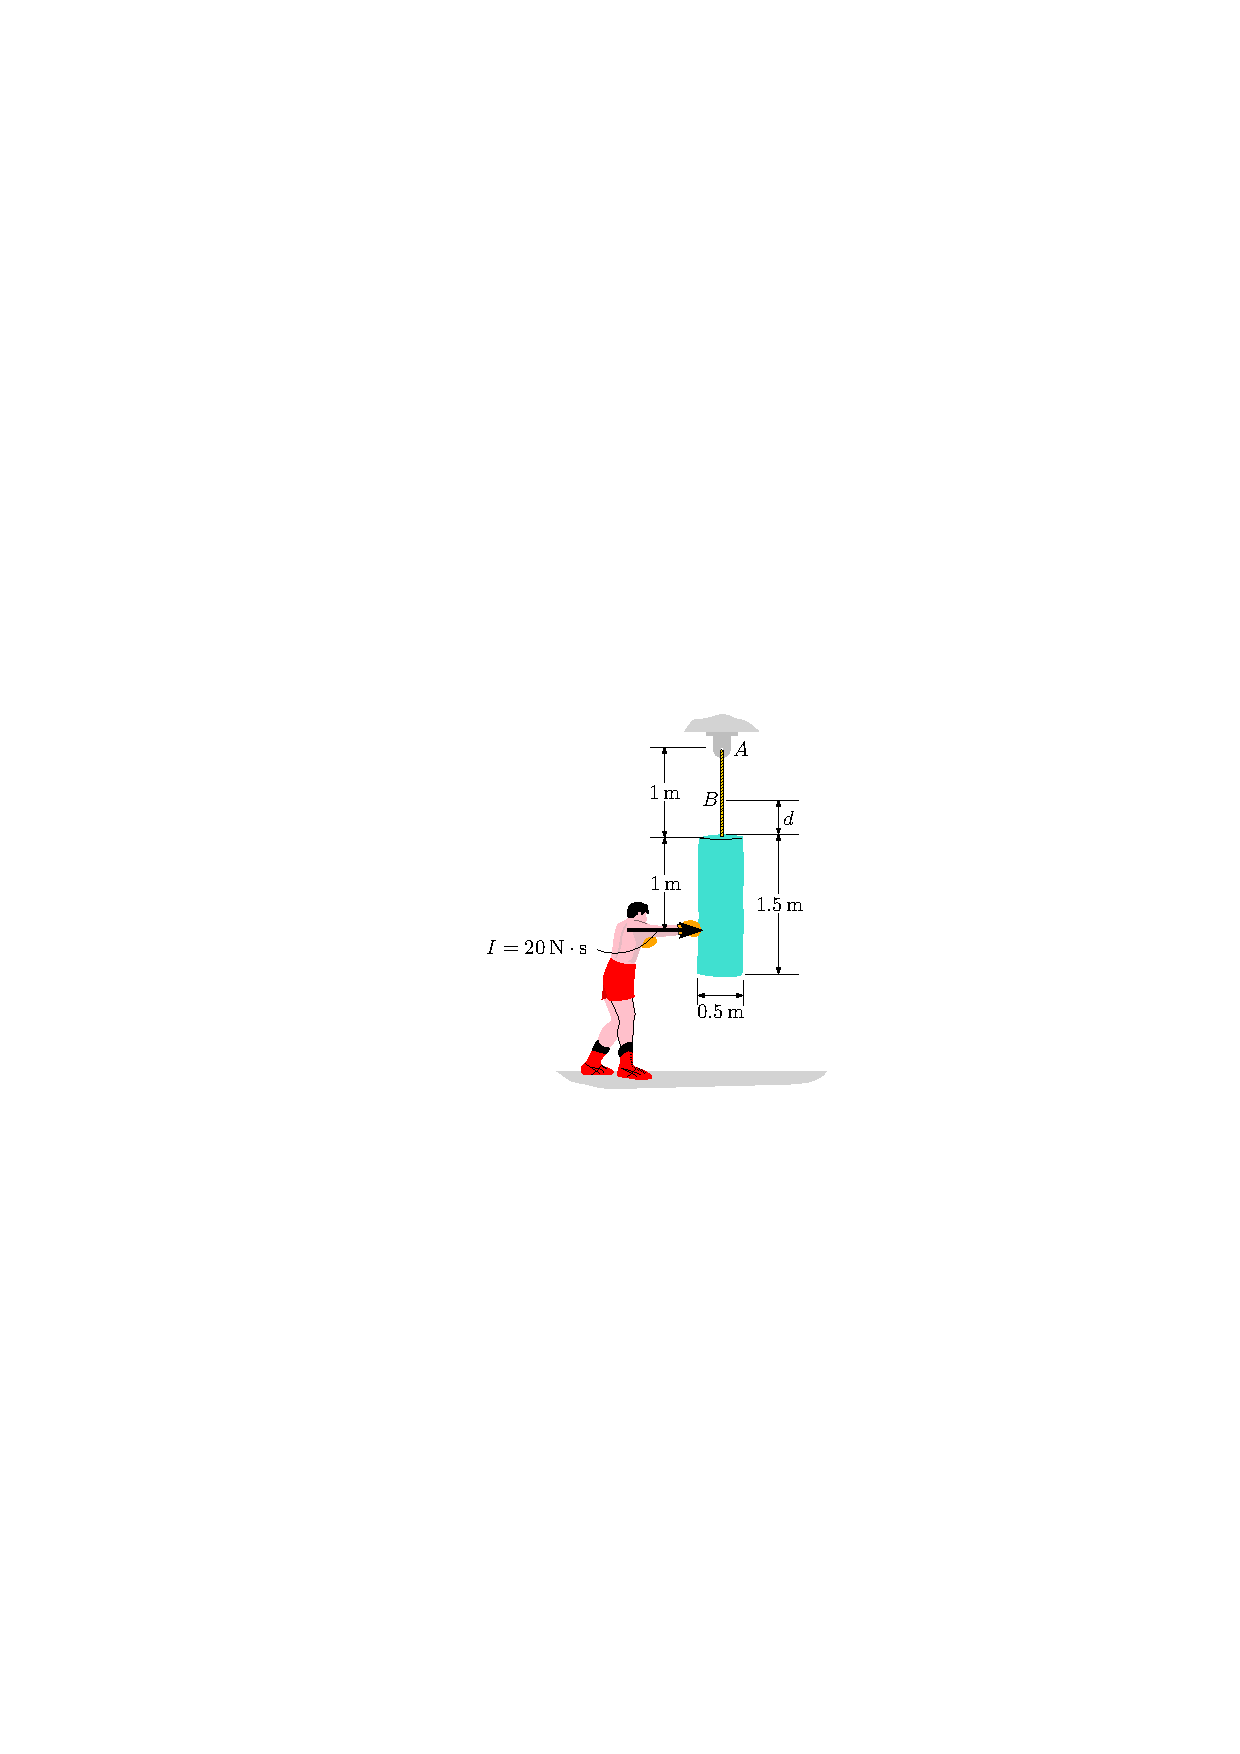
\includegraphics[scale=1.2]{../../images/draw_3}
	\end{flushleft}

\end{minipage}
\begin{minipage}{.5\linewidth}
	\vspace{-1cm}
	\item Se o boxeador bate no saco de pancada de \SI{75}{\kilogram} com um impulso $I= \SI{20}{\newton\cdot\second}$, determine a velocidade angular do saco imediatamente após ele ser atingido. Determine também a localização $d$ do ponto $B$, em torno do qual o saco parece girar. Trate o saco como um cilindro uniforme.\\
	
	\import{../answers}{answer-5}
\end{minipage}
